\section{Slip length}
\label{sec:slip_length}
\section{Porosity}

\section{Permerability and Darcy's law}
\label{sec:darcy_law}
In 1856, H. Darcy found a linear relation between the pressure difference and the fluid flow rate. This relation is called Darcy's law and tells us what volumetric flow rate \footnote{how many cubic meters of fluid per second} $Q$ we can expect from a incompressible liquid with dynamic viscosity $\mu$ through a material with \textit{permeability} $k$ of length $L$ and volume $V$ when we apply a pressure difference $\Delta P$, see figure \ref{fig:darcys_law}. 
\begin{figure}[h]
\begin{center}
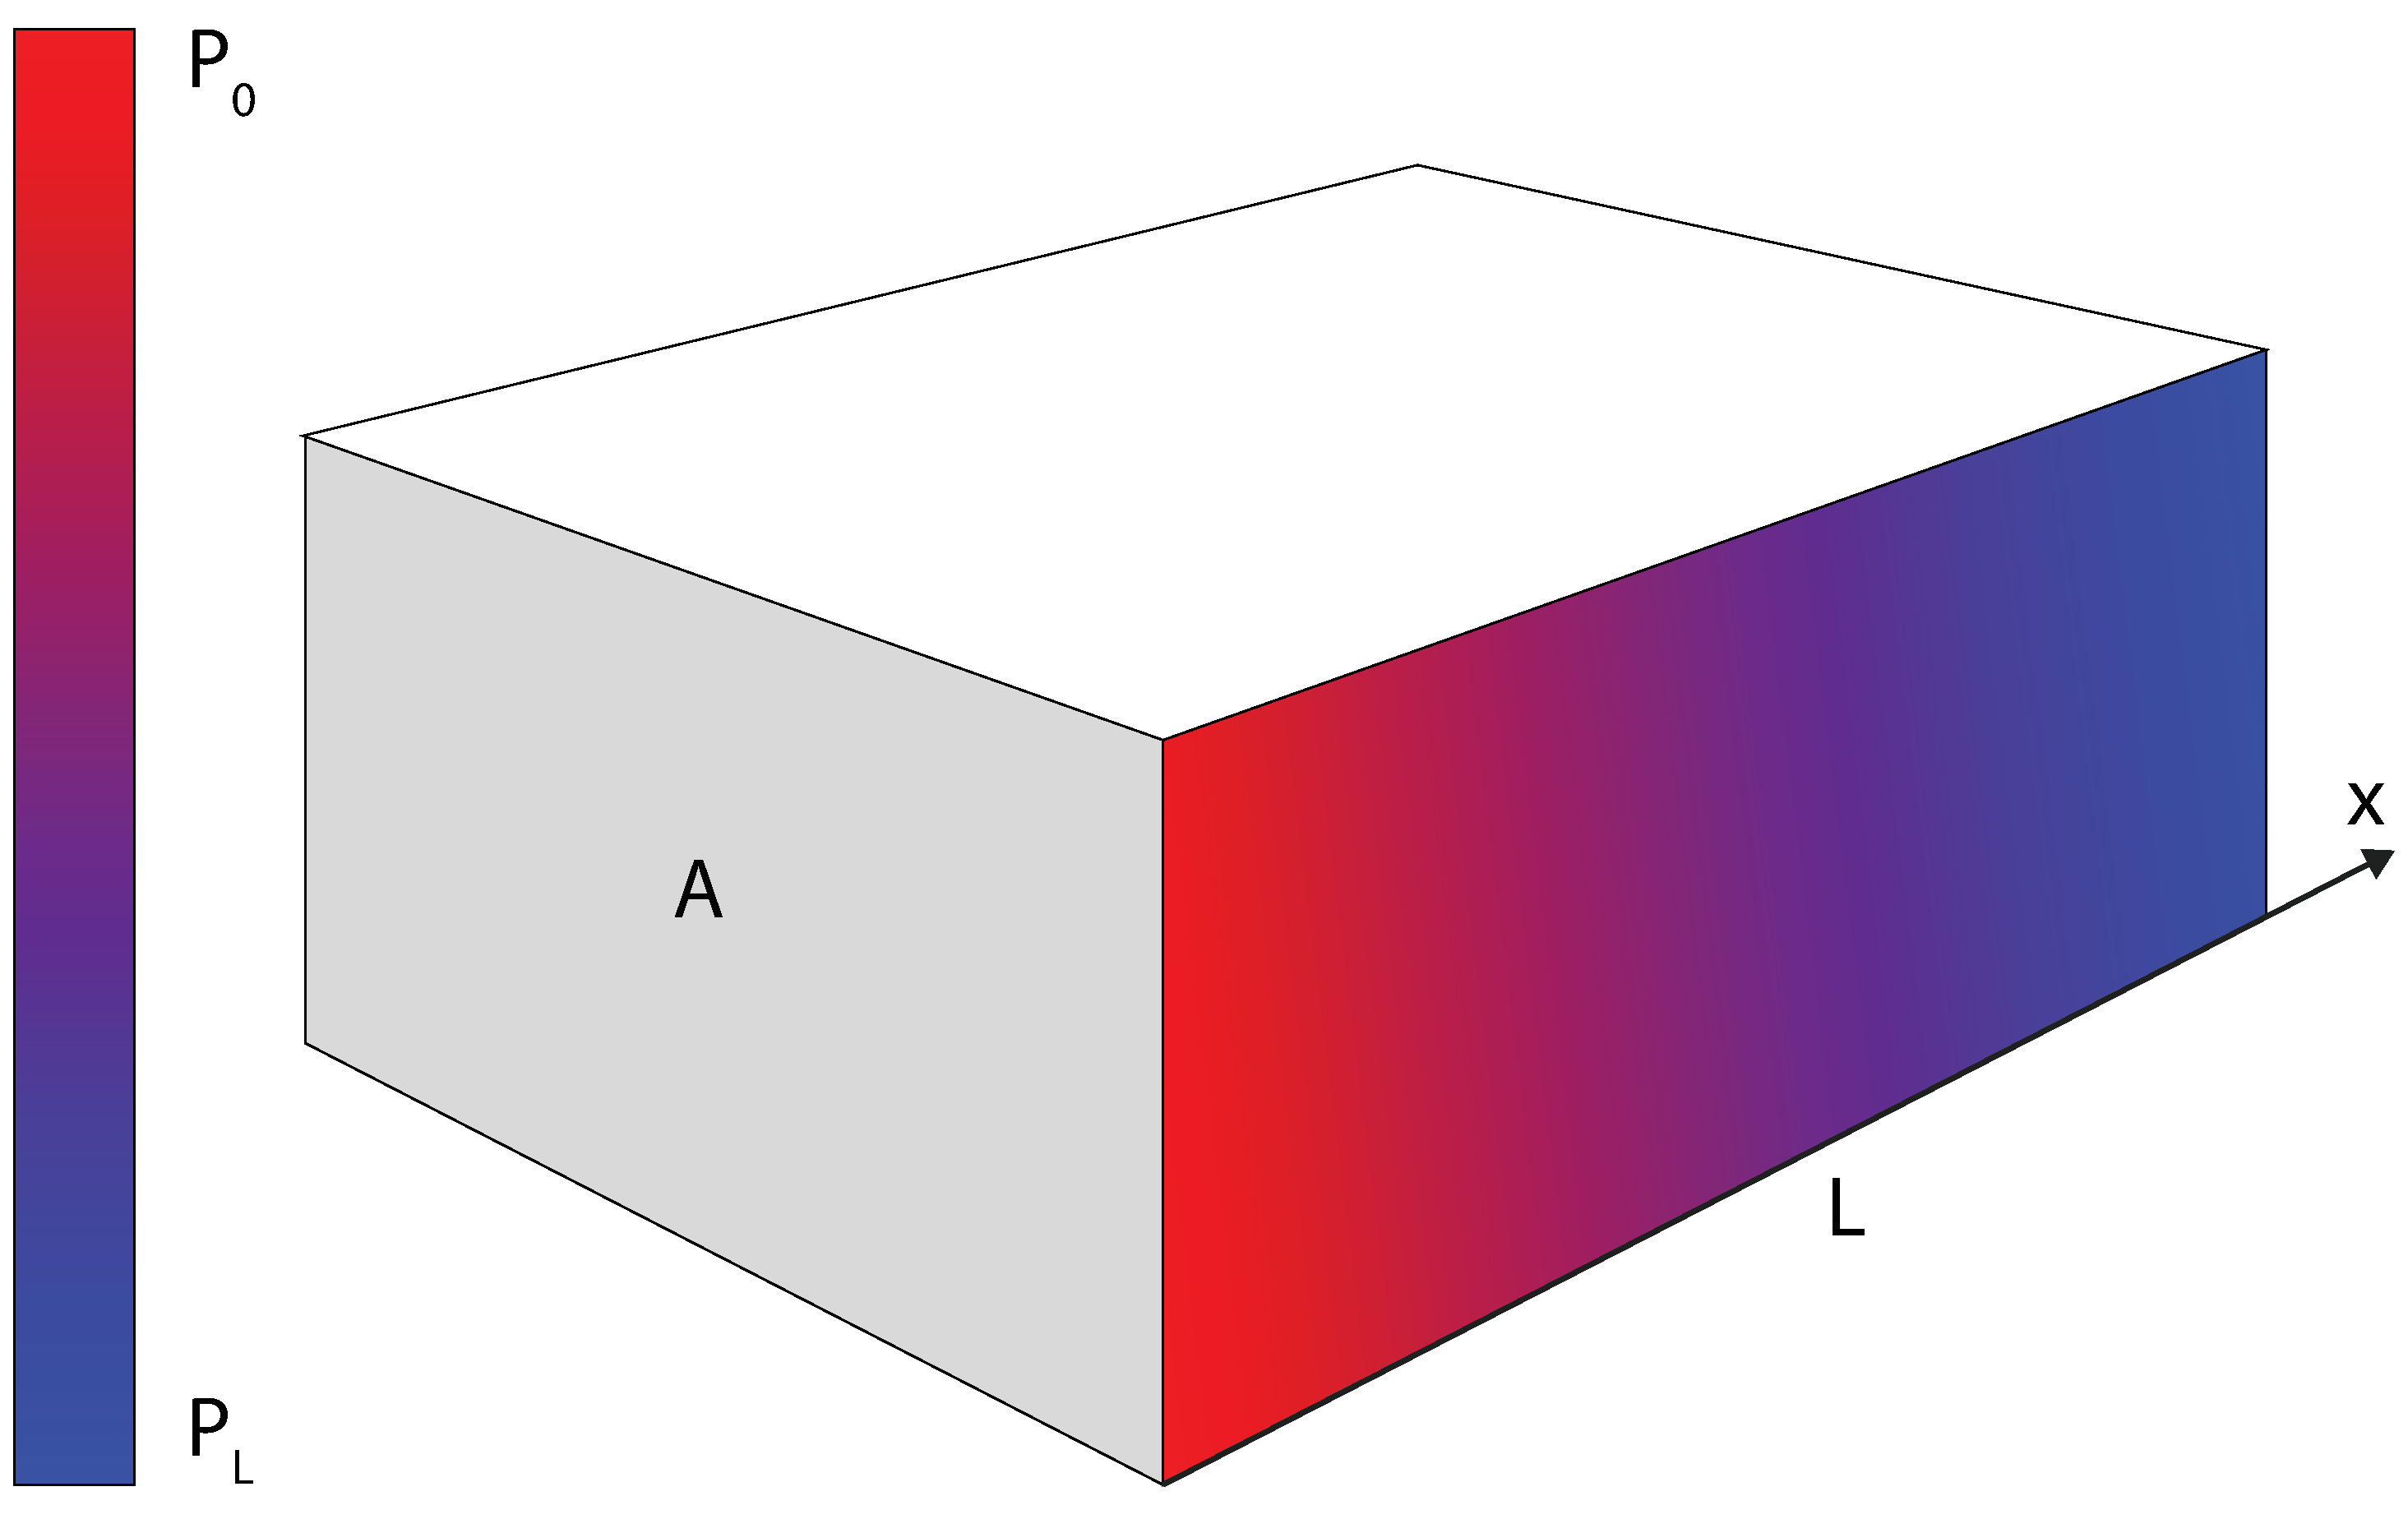
\includegraphics[width=\textwidth, trim=0cm 0cm 0cm 0cm, clip]{kinetic_theory/figures/darcy.eps}
\label{fig:darcys_law}
\end{center}
\caption{A box with volume $V=LA$ with fixed pressure values at $x=0$ and $x=L$. The volumetric flow rate $Q$ through a cross sectional area $A$ is given by Darcy's law.}
\end{figure}
The one dimensional version of Darcy's equation which is given as
\begin{align}
\label{eq:darcy_1}
	Q = A{k\over \mu}{\Delta P\over L},
\end{align}
where $\Delta P = P_0 - P_L \geq 0$, $A$ is the cross sectional area; the area of the material orthogonal on the flow direction. By letting $L\rightarrow 0$, we get the differential form of Darcy's law
\begin{align}
\label{eq:darcy_2}
	Q = -A{k\over \mu}{dP\over dx},
\end{align}
where we picked up a minus sign because the fluid flows from high pressure to low pressure. Darcy's law can be written in a form analogous to Ohm's law
\begin{align}
	u = \sigma_D \nabla P,
\end{align}
where $\sigma_D=k/\mu$ can be seen as a \textit{specific liquid conductivity} of the material. We see the similarities to Ohms law ($J$ being the current density and $E$ the electric field, both measured at the same point $x$) 
\begin{align}
	J = \sigma E.
\end{align}
\subsection{Permeability $k$}
The motivation of introducing the concept permeability is to separate the conductivity parameter $\sigma_D$ into two parts; one that depends on the liquid only, the viscosity $\mu$, and a material specific constant $k$ which we call permeability. This means that we can do an experiment with a liquid with known viscosity, say water, and measure the permeability of some material (Darcy studied a sand filled cylinder in his original experiment). Once you know the permeability, you are able to predict the flow rate through the material for \textit{any} other liquid if you just know the viscosity.\\
This is of course not completely true for all fluids. While Darcy originally found the relation as an empiric equation based on experiments, it can be derived from the Navier-Stokes equations. Darcy's law is only correct if the liquid flow satisfies the no-slip boundary condition. As discussed in section \ref{sec:slip_length}, the velocity of a fluid near the surface is proportional to the mean free path $\lambda$, and is often a non-zero quantity in dilute gases. 
\subsection{Knudsen number}
The Knudsen number is a dimensionless quantity defined as the ratio between the mean free path $\lambda$ and some characteristic length in the material \footnote{such as pore radius $r$} $L$
\begin{align}
	\text{Kn} = \frac{\lambda}{L}.
\end{align}
In the limit of very large Knudsen numbers (Kn$\geq 10$), the mean free path is so large that atoms collide with the surface more often than with each other. 
\subsection{Flow regimes}


\subsection{Klinkenberg effect}
In 1941, L.J. Klinkenberg published a paper explaining the discrepancies between Darcy's law and experiment by applying the theory of no-slip \cite{klinkenberg1941permeability}. He introduced a linear scaling function $f_c$ that relates what he called the \textit{absolute permeability} $k_\infty$, the permeability that is measured with a liquid or a high density gas, to the \textit{apparent permeability} $k_a$ which is the permeability that satisfies Darcy's law. The relation is given as
\begin{align}
	k_a = f_c k_\infty = \left(1 + 4c\text{Kn}\right)k_\infty,
\end{align}
where $c\approx 1.11$ is the no-slip factor in equation \eqref{eq:noslip}. We can rewrite Klinkenberg's equation to 
\begin{align}
	k_a = \left(1 + {b\over P}\right)k_\infty,
\end{align}
by using that
\begin{align}
	4c\text{Kn} &= {4c\lambda \over L} = {b\over P},
\end{align}
where $b=4c\lambda P / L$ is called Klinkenberg's gas slippage factor. We see that $b$ is a constant depending on the geometry of the material and the pressure. In experiments, details about the underlying geometry is often unavailable, so other forms have been suggested \cite{ziarani2012knudsen}.
\subsection{Knudsen's correction}

